%!TEX root = Thesis.tex

\chapter{Coordination Complexes with Silver}
\chaptermark{Silver}
\label{ch:silver}

Silver is as a precious metal that has been used in coins, jewellery and other ornamentation at least since 4000\BC.  Silver salts have a wide range of applications, such as photographic film, wound dressings, and water storage tanks.\cite{Enghag2004Ag}  Silver coordination complexes are also biologically active: bis-diphosphine silver complexes show anti-tumour and anti-fungal activity.\cite{Berners-Price1988, Liu2008}  Metallic silver is used industrially as a catalyst for the conversion of ethene to ethylene glycol, and silver salts are occasionally used as co-catalysts in cross-coupling reactions.\cite{Suzuki1999}  Complexes of silver have been used as catalysts in a number of transformations, including Si-H activation,\cite{Iglesias2012} asymmetric aldol conversions \cite{Sawamura1990} and allylation of benzaldehyde\cite{Malaise2006, Yanagisawa1999}.

% \fixme{find the article from wikipedia to cite here}  Silver coordination complexes have also show biological activity.  \emph{Bis}-diphosphine silver complexes have shown anti-tumour and anti-fungal activity.\cite{Berners-Price1988, Liu2008}

%Silver is used industrially as a catalyst to convert ethene to ethylene glycol on an industrial scale.  It is also often used in the control rods of nuclear reactors.  Silver has also found use as a component in the Oddy test.  This test is used to determine if materials give off gases which may be harmful to art and historical artefacts, specifically the silver is used to detect reduced sulfur and sulfur carbonyl compounds.  \fixme{this needs some citations}

%Furthermore  silver complexes have gained attention recently as potential catalysts in a number of transformations including Si-H activation\cite{Iglesias2012} asymmetric aldol conversions \cite{Sawamura1990} and allylation of benzaldehyde\cite{Malaise2006, Yanagisawa1999}.

Silver coordination chemistry is interesting due to the wide range of different geometries available to the metal, resulting in a high degree of geometrical flexibility. The bite-angle, electronic influence of the diphosphine, and the coordination mode of any ancillary ligands can all impact the type of complex formed.  Possible structures formed for an equimolar reaction of a silver salt with a diphosphine range from the straightforward monometallic complex, to multimetallic clusters with bridging diphosphines (Figure \ref{Silverstructures}).  For a detailed overview of silver coordination chemistry see Meijboom \emph{et al.}\cite{Meijboom2009}

\begin{figure}[h] 
\begin{center}
\vspace{0.5cm}
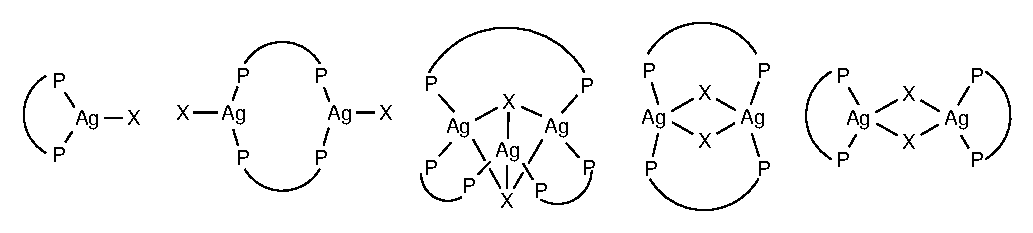
\includegraphics[scale=0.8]{../Figures/Possiblesilverstructures.eps}
\caption[1:1 silver diphosphine complexes]{Possible structures for 1:1 silver diphosphine complexes, reproduced from Meijboom \emph{et al.}\cite{Meijboom2009}}
\vspace{0.2cm}
\label{Silverstructures}
\end{center}
\end{figure}
\vspace{0.2cm}

%In addition to forming unusual coordination environments silver complexes have also been extensively studied due to their biological activity.  Bisdiphosphine silver complexes have shown anti-tumour and anti-fungal activity.\cite{Berners-Price1988, Liu2008} A recent study (Liu2008) showed that silver complexes of bidentate pyridyl phosphines showed in vitro anti-tumour activity.  

Silver complexes with xantphos-derived ligands have been reported previously.\cite{Malaise2006, Balakrishna2008}  In all cases the complexes are monometallic and the majority of these structures are tetrahedral complexes of the type [Ag(xantphos)(NN)] where NN represents a bidentate nitrogen-donor ligand such as 2,2'-bipyridine.  These [Ag(xantphos)(NN)] complexes have been patented for their luminescent properties.\cite{Kobayashi2010, Kobayashi2011a, Kobayashi2012a} Other tetrahedral complexes with \Phxantphos{} include a chelating ligand or two monodentate ligands (Figure \ref{AgPhxantphos}).  Only one trigonal silver \Phxantphos{} complex has been reported (Figure \ref{AgxantphosBr}).\cite{Kaltzoglou2007}.  However, this is likely due to a lack of research rather than synthetic difficulties, as trigonal silver complexes with a chiral xantphos derivative have also been reported.\cite{Malaise2006}

\begin{figure}[htbp]
\centering
\begin{subfigure}[b]{0.3\textwidth}
	\centering
	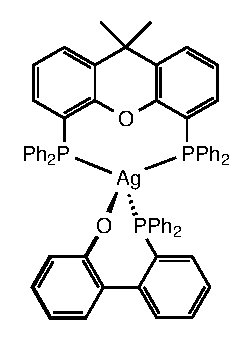
\includegraphics{../Figures/AgxantphosPO.eps}
	\caption{}
	\label{AgxantphosPO}
\end{subfigure}
~
\begin{subfigure}[b]{0.3\textwidth}
	\centering
	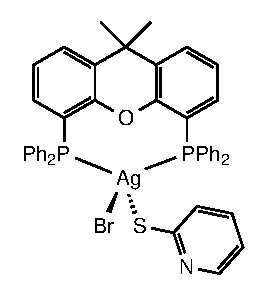
\includegraphics{../Figures/AgxantphosBrSPy.eps}
	\caption{}
	\label{AgxantphosBrSPy}
\end{subfigure}
~
\begin{subfigure}[b]{0.3\textwidth}
	\centering
	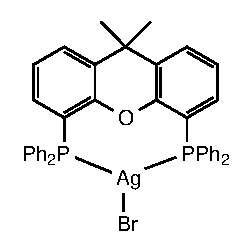
\includegraphics{../Figures/AgxantphosBr.eps}
	\caption{}
	\label{AgxantphosBr}
\end{subfigure}
\\
\caption[Silver \Phxantphos{} complexes]{Tetrahedral and trigonal silver \Phxantphos{} complexes.}
\label{AgPhxantphos}
\end{figure}

%The more flexible backbone of DPEphos allows the formation of triflate or iodide bridged dimers.\cite{Balakrishna2008}, \fixme{find the iodide reference}  Silver complexes of a chiral xantphos derivative \fixme{reference} have also been reported.  

%A trigonal silver complex [AgBr(xantphos)] was synthesised by direct reaction of silver bromide and xantphos in refluxing acetone or acetonitrile.\cite{Kaltzoglou2007}

Crystal structures of [AgBr(\Phxantphos)] (Figure \ref{crystal:AgPhxantphosBr} and [AgBr(Ph-xantphos)(S-pyH)] (\acrshort{py} = \acrlong{py}, Figure \ref{AgxantphosBrHpyS}) have been reported.\cite{Kaltzoglou2007}  In the trigonal structure the P-Ag-P angle is 109.38(7)\degrees{} which increases to 111.507(17)\degrees{} for [AgBr(Ph-xantphos)(S-pyH)].  The natural bite-angle for Ph-xantphos (111.7\degrees)\cite{Birkholz2009} is very close to the observed bite-angle.  Thiopyridine can act as a bidentate chelating ligand, however in this case the thione tautomer is formed and monodentate coordination through the sulfur is observed.  In order for the pyridine thiol to chelate, the P-Ag-P angle would need to decrease significantly.  In this instance the rigidity and steric bulk of Ph-xantphos prevents this from happening.\cite{Kaltzoglou2007}

\begin{figure}[htbp]
\centering
\begin{subfigure}[b]{0.58\textwidth}
	\centering
	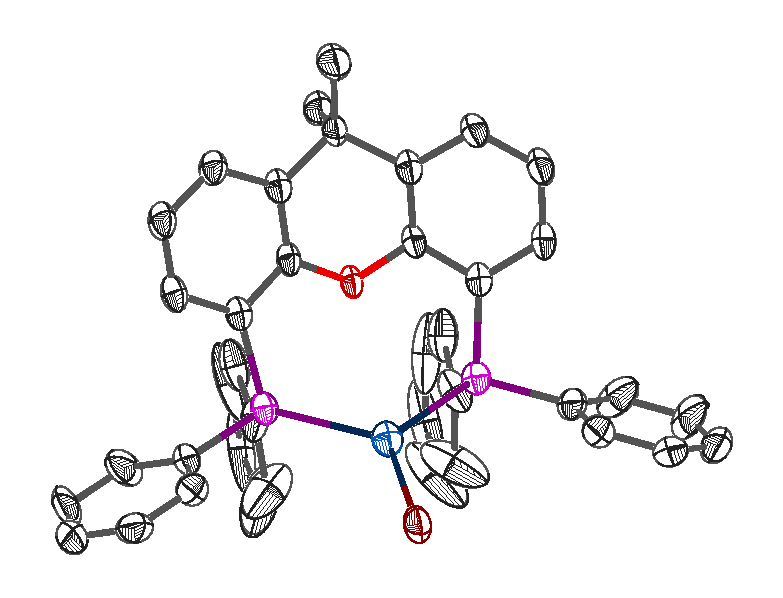
\includegraphics[width=\textwidth]{../Othercrystals/xantsAgBr.eps}	
	\caption{}
%	\label{crystal:AgxantphosBr}
\end{subfigure}
~
\begin{subfigure}[b]{0.36\textwidth}
	\centering
	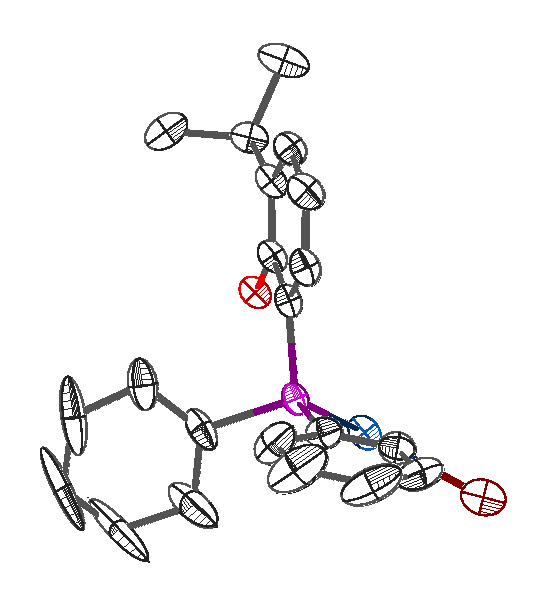
\includegraphics[width=\textwidth]{../Othercrystals/xantsAgBrside.eps}
	\caption{}
%	\label{crystal:AgxantphosBrside}
\end{subfigure}
\\
\caption[X-ray crystal structure of AgBr(Ph-xantphos)]{X-ray crystal structure of [AgBr(Ph-xantphos)] showing the front (a) and side (b).\cite{Kaltzoglou2007}  Hydrogen atoms omitted for clarity.}\label{crystal:AgPhxantphosBr}
\end{figure}

\begin{figure}[htb] 
\begin{center}
\vspace{0.5cm}
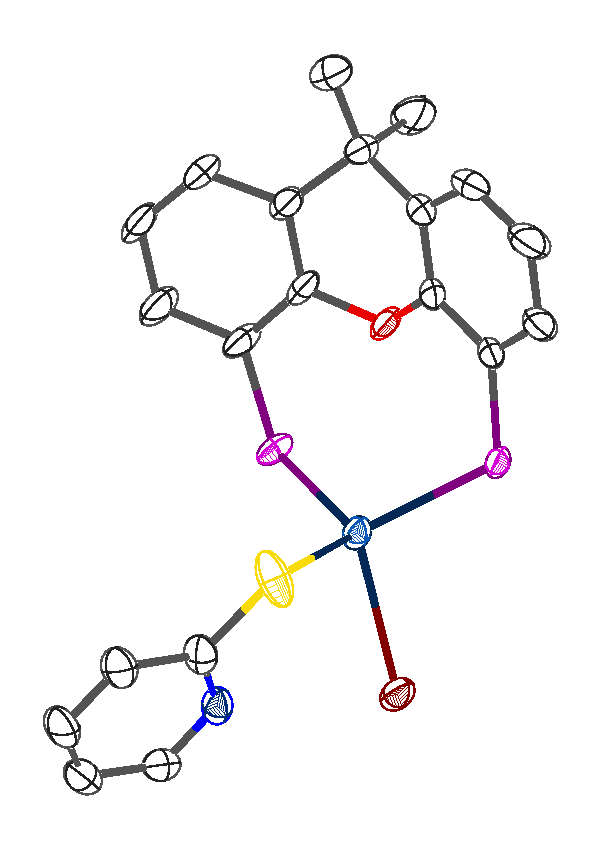
\includegraphics[width=0.45\textwidth]{../Othercrystals/AgxantphosBrHpyS.eps}
\caption[ORTEP diagram of Ag(Ph-xantphos)(HpyS)Br]{ORTEP diagram of [Ag(Ph-xantphos)(HpyS)Br].\cite{Kaltzoglou2007} Phenyl rings and hydrogen atom omitted for clarity}
\vspace{0.2cm}
\label{AgxantphosBrHpyS}
\end{center}
\end{figure}
\vspace{0.2cm}

%The reported complexes are all trigonal geometries with the general formula \ce{[Ag(diphosphine)X]} where X = a negatively charged ligand OTf-, BF4 for Malaise2006.  Of most relevance to this work is the complex [AgBr(xantphos)] reported by Kaltzoglou.\cite{Kaltzoglou2007}  This complex exists as a monomeric species with a P-Ag-P angle of 109.38\degrees{}, very close to the natural bite-angle for xantphos (111.7\degrees).\cite{Kranenburg1995}  The complex reacted with a heterocyclic thione forming the tetrahedral species [AgBr(xantphos)(py2SH)].  The P-Ag-P angle for this is increased slightly to 111.51\degrees{}.  The steric bulk of the xantphos ligand was proposed as the reason for the lack of chelation.\fixme{chelation SN}

%\fixme{Why don't the commas and full-stops look nice under the degrees symbol?}

Silver is an excellent metal for investigating the coordination chemistry of xantphos ligands because 
it forms a wide range of different coordination geometries and has been shown to coordinate \Phxantphos{} close to its natural bite-angle.\cite{Kaltzoglou2007}  There are also a number of potential applications for silver complexes, such as catalysis, biological activity, and luminescent membranes.  Silver is also especially suitable for study using \proton{}, \carbon{}, and \phosphorus{} NMR spectroscopy as both of its isotopes, \Agseven{} and \Agnine{}, are spin \nicefrac{1}{2}, allowing further information to be obtained from the value of the silver-atom coupling constants.  

This chapter presents a study of the reactivity of the \tBusixantphos, \tButhixantphos, and \tBuxantphos{} ligands with two silver precursors: silver chloride and silver tetrafluoroborate.

\section{Silver Chloride Complexes}
\label{section:AgCl}

Silver chloride complexes were synthesised by addition of each of the \tBuxantphos{} ligands to a suspension of silver chloride in chloroform-d (Scheme \ref{Silverchloride}), resulting in [AgCl(diphosphine)] complexes.  In all cases, mass spectrometry showed a clear peak for \ce{[M-Cl]+} with no peaks observed for dimers or higher oligomers.  The \phosphorus{} NMR spectra (see Figure \ref{NMRAgCl} for an example) showed the expected pair of doublets in all cases, as summarised in Table~\ref{table:silverchlorides}.  No relationship was observed between the natural bite-angle and the values of \JAgP.  However, the change in the phosphorus chemical shift upon coordination ($\Delta\delta$) increases with decreasing bite-angle.  This indicates that the decrease in shielding is larger for smaller bite-angles.

%As discussed in Section \ref{section:ligandsynthesis}, the uncoordinated \tBuxantphos{} ligands exhibit \ce{X18A}A'\ce{X18}' spin systems for the \tBu{} protons owing to through-space coupling of the phosphorus atoms, which is larger for the smaller bite-angle ligand \tBusixantphos{}.  Hence the phosphorus atoms are less shielded in \tBusixantphos{} than in \tButhixantphos{} which is less shielded than \tBuxantphos.  However, when the ligands coordinate to the silver atom the through-space coupling is disrupted and is instead replaced by coupling across the silver.  

\begin{scheme}[htbp]
\begin{center}
\vspace{0.5cm}
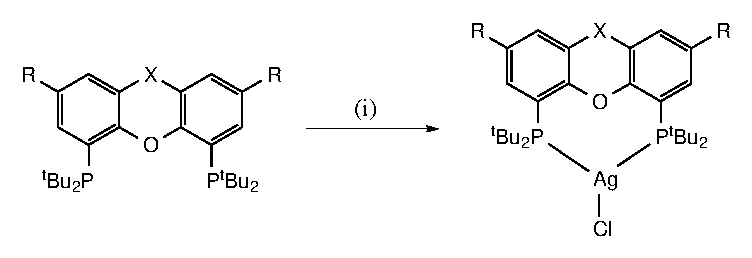
\includegraphics{../Schemes/Silverchloridescheme.eps}
\caption[Synthesis of [Ag(\tBuxantphos)Cl{]} complexes]{Synthesis of [Ag(\tBuxantphos)Cl{]} complexes.}
\vspace{0.2cm}
\label{Silverchloride}
\end{center}
\end{scheme}
\vspace{0.2cm}

\begin{figure}[htbp] 
\begin{center}
\vspace{0.5cm}
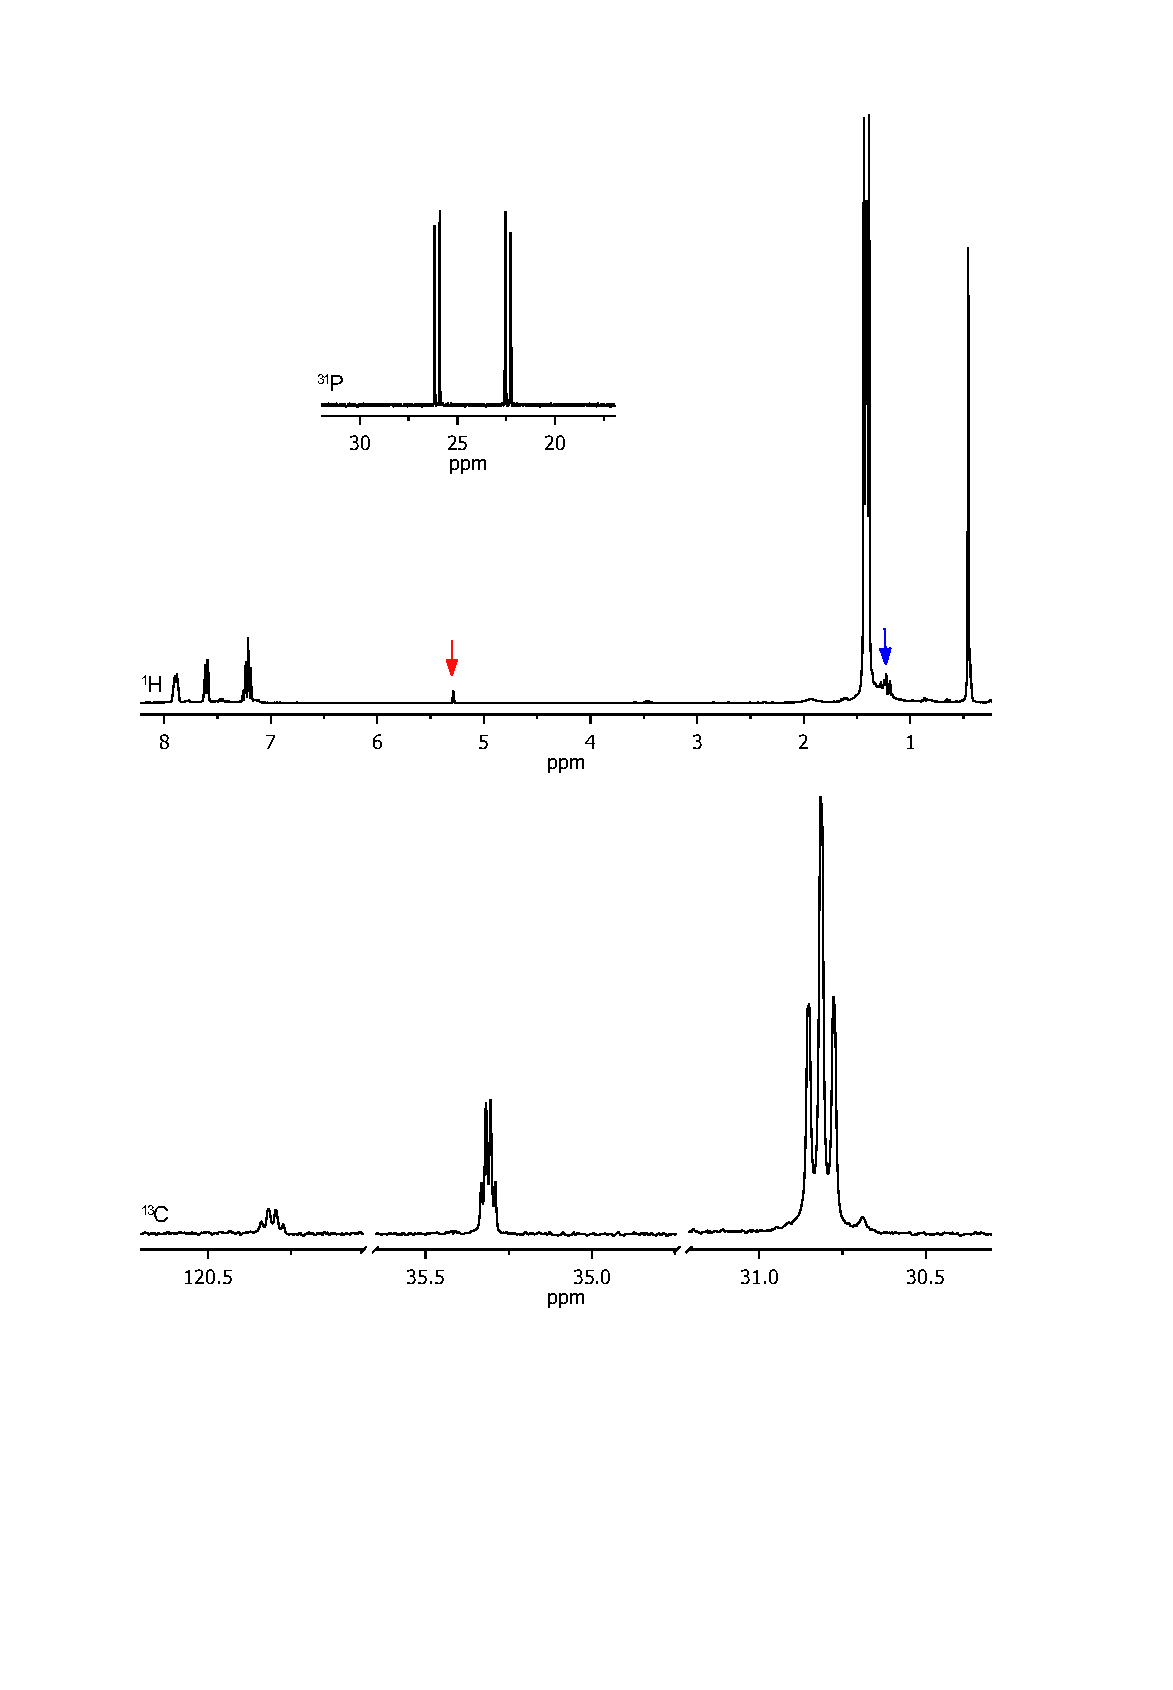
\includegraphics[trim = 2cm 6cm 2cm 2.5cm, clip]{../NMR/SitBuAgCl.eps}
\caption[NMR spectra for {[}Ag(\tBusixantphos)Cl{]}]{\phosphorus{}, \proton{} and \carbon{} NMR spectra of {[}Ag(\tBusixantphos)Cl{]} in \ce{CDCl3}. Arrows indicate impurities, \ce{CH2Cl2} indicated in red.}
\vspace{0.2cm}
\label{NMRAgCl}
\end{center}
\end{figure}
\vspace{0.2cm}

\begin{table}[htbp]
\caption[Selected NMR data of [Ag(\tBuxantphos)Cl{]} complexes]{Selected NMR data of [Ag(\tBuxantphos)Cl] complexes.} 
\vspace{1em}
\label{table:silverchlorides}
\small
\begin{center}
\begin{tabular}{l c c c c}
	\toprule{}
	\bfseries{Compound}&\bfseries{$\delta$\phosphorus{}$/$ppm}&\bfseries{$\Delta\delta/$ppm}&\bfseries{\JAgPseven{}$/$Hz}&\bfseries{\JAgPnine{}$/$Hz}\\
	\midrule{}
	~\tBuSixantphos	&	24.2	&	15.8	&	408.1	&	471.1\\
	~\tBuThixantphos	& 	21.8	&	12.3	&	406.7	&	469.6\\
	~\tBuXantphos		&	20.7	&	10.5	&	409.3	&	472.2\\
	\bottomrule{}
\end{tabular}
\end{center}
\end{table}

The \proton{} NMR spectra for the [Ag(\tBuxantphos)Cl] complexes show half the expected number of aromatic signals, and one signal for the methyl groups and another for the \tBu{} substituents, indicating a complex with planes of symmetry in line with the backbone and perpendicular to it, running through the bridging atoms and the silver (representative spectrum for [Ag(\tBusixantphos)Cl], Figure \ref{NMRAgCl}).  The \tBu{} protons appear as a second order multiplet of the \ce{X18A}A'\ce{X18}' type, similar to the free ligand.  The \carbon{} NMR spectra of the three complexes display some very distinctive signals (representative example, [Ag(\tBusixantphos)Cl], Figure \ref{NMRAgCl}, bottom).  The \emph{ipso} phosphorus carbon on the aryl ring and the quaternary \tBu{} carbon appear as apparent quartets, while the signal for the terminal \tBu{} carbons is an apparent triplet of doublets.  For each of these signals we would expect a doublet of virtual triplets or virtual triplet of doublets for each of the silver isotopologues.  Owing to this complex spin system values for the individual coupling constants were unable to be determined.  The spectroscopic data for the three [Ag(\tBuxantphos)Cl] complexes show significant similarities, with no major discrepancies, indicating that all three complexes have the same overall geometries with only subtle differences.  

%Similar complexes to \fixme{insert reference to the xantphos one} were synthesised for the sulfur, silicon and carbon bridged tBu-xantphos ligands.  The ligands were reacted with silver chloride in the dark and generated the expected [AgCl(L)] complexes.  The \phosphorus{} NMR spectra showed the expected pair of doublets in all cases as summarised in Table~\ref{table:silverchlorides}.  All had mass spectra that showed a clear peak for [M-Cl-]+ with no sign of any dimeric species, clearly indicating a monomeric species.  

Colourless crystals of [Ag(\tButhixantphos)Cl] suitable for single-crystal X-ray diffraction were obtained by inwards diffusion of \ce{Et2O} into a \ce{CH2Cl2} solution of the complex.  The crystal structure is shown in Figure \ref{Crystalthixantphossilverchloride}, confirming the proposed monomeric trigonal structure.  Selected bond lengths and angles, and crystallographic data are given in Tables \ref{table:crystalthixantphossilverchloride:lengths} and \ref{table:crystalthixantphossilverchloride:data} respectively.  [Ag(\tButhixantphos)Cl] crystallised in the P2\sub{1} space group, while the similar complex [AgBr(Ph-xantphos)] crystallised in the higher symmetry P2\sub{1}/\emph{m} space group.\cite{Kaltzoglou2007}  The P-Ag-P angle of 130.50(7)\degrees{} is larger than the bite-angle for [AgBr(Ph-xantphos)] (109.37(1)\degrees{}).  The silver oxygen distance of 3.007(6) \si{\angstrom} indicates there no interaction between these atoms.
\fixme{compare to the natural bite-angle once obtained} 

\begin{figure}[htbp]
\begin{center}
\vspace{0.5cm}
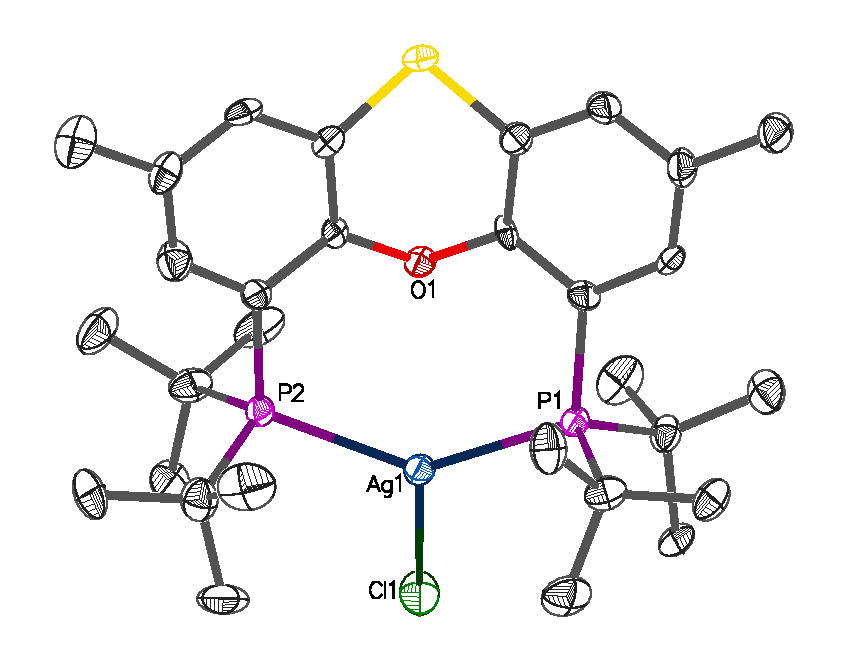
\includegraphics[scale=0.8]{../Figures/Crystalthixantphossilverchloride.eps}
\caption[X-ray crystal structure of [Ag(\tButhixantphos)Cl{]}]{X-ray crystal structure of [Ag(\tButhixantphos)Cl], hydrogen atoms omitted for clarity.}
\vspace{0.2cm}
\label{Crystalthixantphossilverchloride}
\vspace{0.2cm}
\end{center}
\end{figure}
\vspace{0.2cm}



%Silver thixantphos chloride was successfully crystallised as colourless crystals in the \fixme{P21} space group (Figure \ref{crystalthixantphossilverchloride}).  Selected bond lengths and angles, and crystallographic data are given in Tables \ref{table:crystalthixantphossilverchloride:lengths} and \ref{table:crystalthixantphossilverchloride:data} respectively.  The X-ray crystal structure shows a trigonal planar structure with the P-Ag-P angle of 130.4\degrees moderately distorted from the ideal trigonal planar structure.  The Ag-O distance is well outside the sum of the van der waals radii indicating no interaction between the two atoms.  The bite-angle is very close to the natural bite-angle calculated for tBu-thixantphos as 131.4\degrees.  As such the coordination geometry is likely driven very much by ligand effects rather than the silver or the chloride.  Silver can form a huge array of different coordination geometries and generally the preferred structure is controlled by ligand effects.\fixme{get a citation}



\begin{figure}[htbp]
\begin{center}
\vspace{0.5cm}
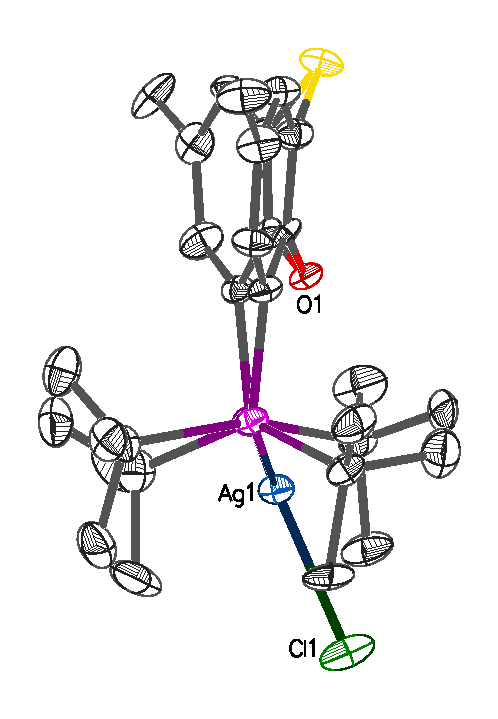
\includegraphics[scale=0.8]{../Figures/Crystalthixantphossilverchloridesideview.eps}
\caption[X-ray crystal structure of [Ag(\tButhixantphos)Cl{]}, side view]{X-ray crystal structure of [Ag(\tButhixantphos)Cl], side view.}
\vspace{0.2cm}
\label{Crystalthixantphossilverchloride:sideview}
\end{center}
\end{figure}
\vspace{0.2cm}

\begin{table}[htbp]
\caption[Selected bond distances and angles of [Ag(\tButhixantphos)Cl{]}]{Selected bond distances (\AA) and angles (\degrees) of [Ag(\tButhixantphos)Cl]}
\vspace{1em}
\label{table:crystalthixantphossilverchloride:lengths}
\small
\begin{center}
\begin{tabular}{l l l l}
	\toprule
	\multicolumn{2}{l}{\bfseries{~Bond distances (\si{\angstrom})}} & \multicolumn{2}{c}{\bfseries{Bond angles (\degrees)}} \\
	\midrule		
	~P1-P2		~~&~~4.416(3)~~	&~~P1-Ag1-P2			&~~130.50(7)~~	\\	
	~P1-Ag		~~&~~2.430(2)~~	&~~P1-Ag1-Cl1			&~~116.46(8)~~	\\
	~P2-Ag		~~&~~2.433(2)~~	&~~P2-Ag1-Cl1			&~~112.95(8)~~	\\
	~Ag-O1		~~&~~3.007(6)~~	&~~Aryl ring 1-Aryl ring 2		&~~35.7(3)~~		\\
	~Ag-Cl1		~~&~~2.491(2)~~	&~~					&~~		~~		\\
	\bottomrule{}
\end{tabular}
\end{center}
\end{table}

\begin{table}[htbp]
\small
\caption[Crystallographic data for [Ag(\tButhixantphos)Cl{]}]{Crystallographic data and structure refinement for [Ag(\tButhixantphos)Cl]} 
\vspace{1em}
\label{table:crystalthixantphossilverchloride:data}
\small
\begin{center}
\begin{tabular}{l l}
	\toprule
	\bfseries{Empirical formula}~~& \bfseries{\ce{C30H46AgClOP2S}}\\
	\midrule
	Formula weight	 							& 659.99\\
	Temperature/K	 							& 285.47(10)\\
	Crystal system	 							& monoclinic\\
	Space group	 							& P2\sub{1}\\
	a$/$\si{\angstrom}							& 8.6697(3)\\
	b$/$\si{\angstrom} 							& 15.4417(6))\\
	c$/$\si{\angstrom}							& 11.9482(4)\\
	$\alpha/$\degrees							& 90\\
	$\beta/$\degrees							& 99.700(3)\\
	$\gamma/$\degrees							& 90\\
	Volume$/$\si{\angstrom\cubed}  				& 1576.70(10)\\
	Z	 									& 2\\
$\rho$\sub{calc} \si{\milli\gram}$/$\si{\milli\metre\cubed} 	& 1.390\\
\si{\metre}$/$\si{\milli\metre} 						& 7.636\\
F(000)	 									& 688.0\\
Crystal size$/$\si{\milli\metre\cubed}	 				& 0.3842 x 0.3421 x 0.1062\\
Radiation	 									& CuK$\alpha$ ($\lambda$ = 1.54184)\\
2$\theta$ range for data collection					& 7.506 to 147.890\degrees\\
Index ranges	 								& -10 $\leq$ h $\leq$ 10, -19 $\leq$ k $\leq$ 16, -14 $\leq$ l $\leq$ 14\\
Reflections collected	 							& 12454\\
Independent reflections	 						& 5818 [R\sub{int} = 0.0724, R\sub{sigma} = 0.0651]\\
Data$/$restraints$/$parameters					& 5818$/$1$/$339\\
Goodness-of-fit on F$^{2}$	 					& 1.138\\
Final R indexes [I$>$=2$\sigma$ (I)]	 				& R\sub{1} = 0.0545, wR\sub{2} = 0.1579\\
Final R indexes [all data]	 						& R\sub{1} = 0.0563, wR\sub{2} = 0.1618\\
Largest diff. peak/hole / e \si{\per\angstrom\cubed}		& 0.88/-1.78	\\
Flack parameter								& -0.016(13)	\\
	\bottomrule
\end{tabular}
\end{center}
\end{table}

A side view of [Ag(\tButhixantphos)Cl] given in Figure \ref{Crystalthixantphossilverchloride:sideview} shows the P-Ag-Cl angle relative to the ligand backbone.   The chloride is not centred, with a difference in the P-Ag-Cl angles of 3.49\degrees.  This difference is likely the result of the backbone twisting with the chloride occupying the least sterically hindered site.  The backbone is bent, resulting in two distinct faces of the molecule.  In [Ag(tBu-thixantphos)Cl] the chloride sits on the convex face of the ligand while in [AgBr(Ph-xantphos)] (Figure \ref{crystal:AgPhxantphosBr}) the bromide ligand occupies the concave face.\cite{Kaltzoglou2007}  In addition, the C(aryl)-P-Ag-Cl dihedral angles of 159.8(3)\degrees{} and 147.4(3)\degrees{} in [Ag(\tButhixantphos)Cl] are significantly larger then the corresponding dihedral angles in [Ag(Ph-xantphos)Br] of 109.6(4)\degrees{}.  The difference in the coordination plane between the two complexes, is likely the result of the steric influence of the \tBu{} groups compared to the phenyl rings; the chloride sits below the \tBu{} groups while intercalating with the phenyl rings.  The backbone bending would result in two different sets of \tBu{} groups, which would have different NMR properties.  However, this is not apparent in the NMR spectra of any of the [Ag(\tBuxantphos)Cl] complexes (Figure \ref{NMRAgCl}) indicating that the backbone is likely inverting rapidly in solution (Scheme \ref{Aginversion}).  

\begin{scheme}[htbp]
\begin{center}
\vspace{0.5cm}
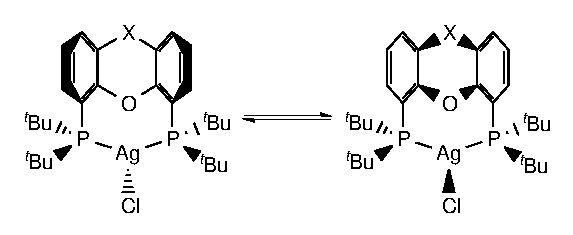
\includegraphics{../Schemes/Silverinversion}
\caption[Inversion of the xantphos backbone in [Ag(\tBuxantphos)Cl{]}]{Inversion of the xantphos backbone in [Ag(\tBuxantphos)Cl].}
\vspace{0.2cm}
\label{Aginversion}
\vspace{0.2cm}
\end{center}
\end{scheme}
\vspace{0.2cm}

%In the solid state structure of silver tBu-thixantphos chloride the backbone shows a significant degree of twisting \fixme{get some info about how much twisting is present} and is bent to give two distinct halves of the molecule.  The chloride is on the convex side of the molecule rather than the \fixme{less sterically hindered - check this} concave side and is not perfectly centred with a difference in the P-Ag-Cl angles of 3.49\degrees{}.  This difference is likely due to the backbone twisting and the chloride occupying the least sterically hindered space.  This structure would result in two distinct sets of t-Bu groups, the two on the convex face and the two on the concave face.  However, this is not observed in the NMR spectra.\fixme{the NMR of the tBu is a bit of a mess and I need to look at it again}  This indicates that the backbone is not static in solution but is inverting on the NMR timescale such that the signals for the two t-Bu environments average and only a single t-Bu \proton{} resonance and two t-Bu \carbon{} resonances are observed.  

\section{Reactions with Silver Tetrafluoroborate}

Complexes of the type [Ag(\tBuxantphos)]\ce{BF4} were synthesised in order to investigate the coordination of the diphosphine ligands in the absence of other ligands.  Although tetrafluoroborate can coordinate to silver, it is unusual for it to do so, and numerous examples exist of silver complexes with free coordination sites that have a non-coordinated \ce{BF4-} counterion (Figure \ref{Linearsilver}).\cite{Ainscough2011, Bayler1996, Vlugt2009b}.  Previous reports have shown that in the presence of an ether group and a tetrafluoroborate ion a linear diphosphine complex with mutually \emph{trans} phosphorus atoms and no other ligands was synthesised.\cite{Heuer2000}  In addition, coordination of the tetrafluoroborate the silver will result in a shift of peak in the \fluorine{} NMR spectrum.

\begin{figure}[htbp]
\begin{center}
\vspace{0.5cm}
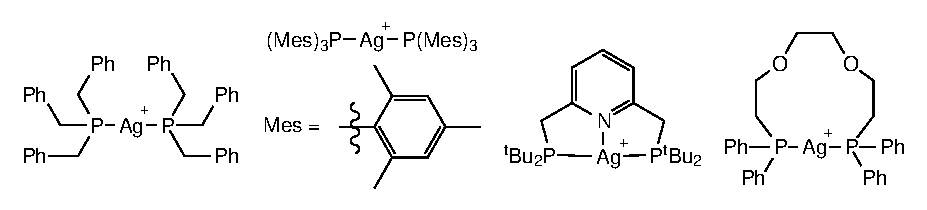
\includegraphics{../Figures/Linearsilvercomplexes.eps}
\caption[Silver complexes with free coordination sites and \ce{BF4-} counterions]{Examples of silver complexes with free coordination sites and non-coordinating \ce{BF4-} counterions.\cite{Ainscough2011, Bayler1996, Vlugt2009b}}
\vspace{0.2cm}
\label{Linearsilver}
\vspace{0.2cm}
\end{center}
\end{figure}
\vspace{0.2cm}

The reaction between \ce{AgBF4} and the \tBuxantphos{} ligands proceeded at room temperature in \ce{CH2Cl2}, going to completion in under one hour (Scheme \ref{SilverBF4}).  The resulting [Ag(\tBuxantphos)]\ce{BF4} complexes are light-sensitive in solution and in \ce{CDCl3} solution completely degraded in 12 hours.  For all three diphosphine ligands the mass spectra show a molecular ion peak corresponding to \ce{[Ag(diphosphine)]+}. In all cases the \phosphorus{} NMR spectra (for an example see Figure \ref{NMRAgBF4}) show the expected pair of doublets, indicating chelation to a single silver atom.  No relationship between the bite-angle and the \JAgPseven{} or \JAgPnine{} coupling constants was observed.  The \JAgPseven{} or \JAgPnine{} coupling constants are larger than those for the silver chloride complexes (Table \ref{table:silverBF4}).  This is consistent with their formulation as two-coordinate silver complexes, as the values of M-P coupling constants for \ce{d^{10}} metals generally increase with decreasing coordination number.\cite{Pregosin2012}

The \fluorine{} NMR spectra of the three [Ag(\tBuxantphos)]\ce{BF4} complexes show a single resonances between -151.3 and -151.9 ppm, indicating non-coordinating \ce{BF4-} counterions.  In the \proton{} NMR spectra the \tBu{} resonances appear as a virtual triplet.  Virtual triplets are commonly observed for X\sub{\emph{n}}AA\textprime{}X\textprime{}\sub{\emph{n}} when A and A\textprime are strongly coupled such that \JXX{AA\textprime{}} is very much larger than the difference between \JXX{AX} and \JXX{AX\textprime{}}.\cite{Harris1964}  In coordination compounds this condition is typically met if the two phosphorus atoms are in a \trans{} configuration resulting in a strong coupling of the spin system.\cite{Pregosin2012}  In this case as the triplet is not a perfect 1:2:1 triplet it is likely that the phosphines are not strictly \trans{} and the P-Ag-P angle is less than 180\degrees{}.  
%With the tBu-xantphos ligands a single resonance in the \fluorine{} NMR spectrum (with two signals due to the \Bten{} and \Beleven{} isotopomers) was observed in the position expected for a non-coordinating \ce{BF4-}.  However no evidence for oxygen coordination was found.  As such it is likely that similar to previous reports the structure is an electron-deficient 14-electron silver diphosphine linear complex.  

\begin{scheme}[h]
\begin{center}
\vspace{0.5cm}
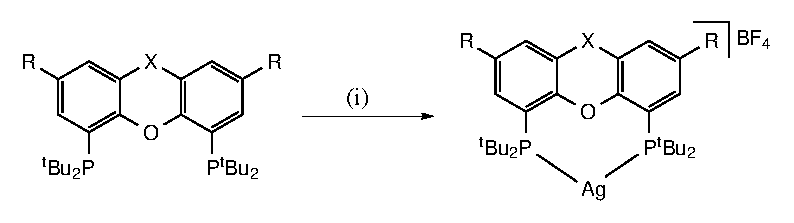
\includegraphics{../Schemes/SilverBF4scheme.eps}
\caption[Synthesis of [Ag(\tBuxantphos){]}\ce{BF4} complexes]{Synthesis of [Ag(\tBuxantphos){]}\ce{BF4} complexes.}
\vspace{0.2cm}
\label{SilverBF4}
\end{center}
\end{scheme}
\vspace{0.2cm}

\begin{figure}[htbp] 
\begin{center}
\vspace{0.5cm}
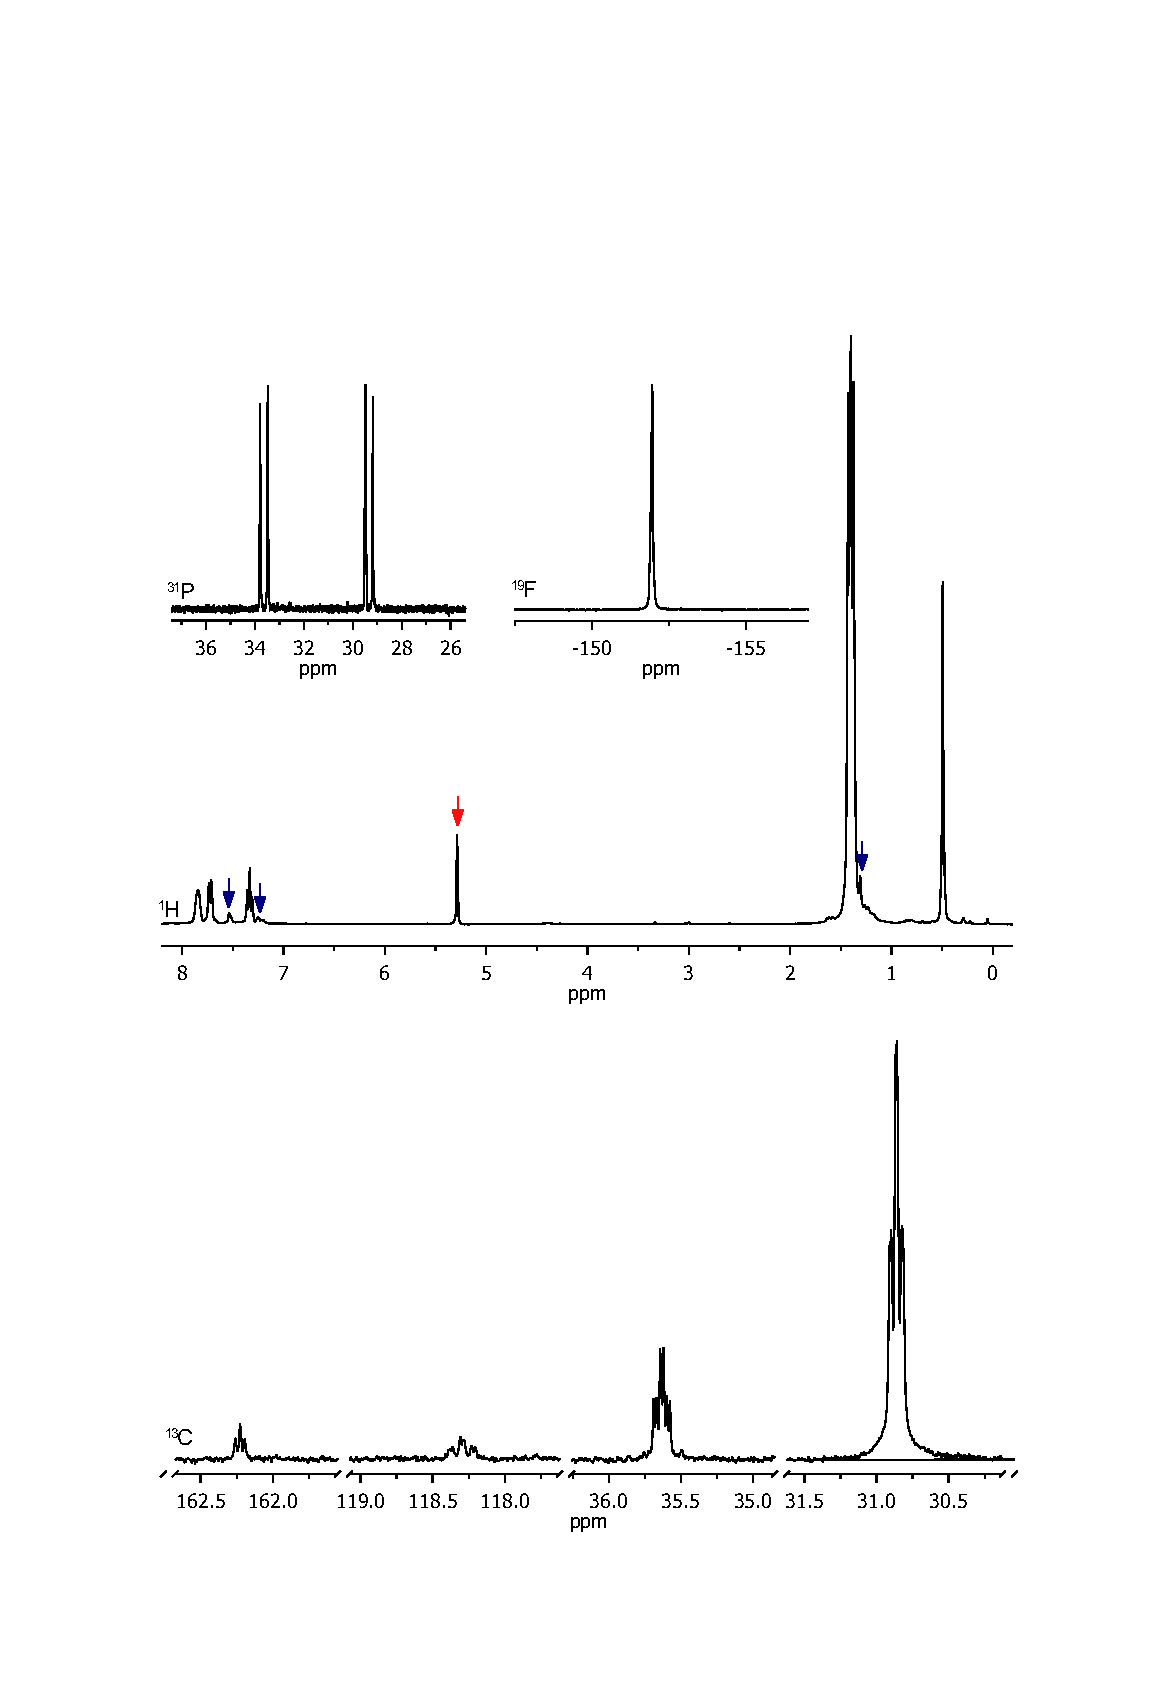
\includegraphics[trim = 2.3cm 2.2cm 2cm 5cm, clip]{../NMR/SitBuAgBF4_2.eps}
\caption[NMR spectra for [Ag(\tBusixantphos){]}\ce{BF4}]{NMR spectra for [Ag(\tBusixantphos)]\ce{BF4} in \ce{CDCl3}.  Arrows indicate impurities, \ce{CH2Cl2} indicated in red.}
\vspace{0.2cm}
\label{NMRAgBF4}
\end{center}
\end{figure}
\vspace{0.2cm}

\begin{table}[h]
\caption[Selected NMR data of [Ag(\tBuxantphos){]}\ce{BF4} complexes]{Selected NMR data of [Ag(\tBuxantphos){]}\ce{BF4} complexes} 
\vspace{1em}
\label{table:silverBF4}
\small
\begin{center}
\begin{tabular}{l c c c c c}
	\toprule{}
	~ & \multicolumn{4}{c}{\bfseries{\phosphorus}} & \bfseries{\fluorine} \\
	\cmidrule(lr){2-5} \cmidrule(lr){6-6}
	\bfseries{Diphosphine}~~&~~\bfseries{$\delta/$ppm}~~&~~\bfseries{$\Delta\delta/$ ppm}~~&~~\bfseries{\JAgPseven{}$/$Hz}~~&~~\bfseries{\JAgPnine{}$/$Hz}~~&~~\bfseries{$\delta/$ppm}~~\\
	\midrule
	\tBuSixantphos 	&~~31.5~~&~~23.1~~&~~482.9~~&~~557.4~~&~~-151.9\\ 
	\tBuThixantphos	&~~28.4~~&~~18.9~~&~~486.7~~&~~562.2~~&~~-151.3\\
	\tBuXantphos		&~~27.6~~&~~17.4~~&~~486.3~~&~~561.1~~&~~-151.9\\
	\bottomrule{}
\end{tabular}
\end{center}
\end{table}

The [Ag(\tBuxantphos)]\ce{BF4} complexes show distinctive peaks in their \carbon{} NMR spectra (see Figure \ref{NMRAgBF4} for a representative example), similar to those observed for the [Ag(\tBuxantphos)Cl] complexes (Section \ref{section:AgCl}).  The most downfield signal is for the aryl carbon attached to the oxygen atom (the \emph{O}-\emph{ipso} carbon).  This signal appears as a virtual triplet, as expected for a XAA'X' system with strongly coupled phosphorus atoms.  The signals for the \emph{ipso} carbon attached to phosphorus, and the \tBu{} quaternary and terminal carbons, all appear as triplets of doublets due to coupling to phosphorus and both isotopes of silver.  These signals would be expected to appear as a pair of virtual triplets of doublets; however, if the two leftmost peaks of one triplet of doublets overlapped with the two central peaks of the other triplet of doublets this could result in an apparent triplet of doublets (assuming that the virtual triplet is not a strict 1:2:1 triplet, which is likely applicable here as the \proton{} NMR signal for the \tBu{} protons was not a 1:2:1 triplet).

The [Ag(\tBuxantphos)]\ce{BF4} complexes have two free coordination sites; however, there is no evidence for either the ligand oxygen atom or the \ce{BF4-} acting as another ligand.  This is likely due to the steric constraints of the larger bite-angle ligands and the bulky \tBu{} groups.  Attempts were made to react the analogous [Ag(\tBuxantphos)]\ce{PF6} complexes with ethene, ethyne and carbon monoxide, however no reactivity was observed.\cite{Bill306}

\subsection{Reactions with LiCCPh}

Silver acetylide complexes have gained attention recently due to their luminescent properties.\cite{Yam1997, Yam1998, Xu2013}  Silver acetylides supported by phosphine ligands tend to form cluster complexes with no monomeric structures currently reported in the \gls{CSD}.\cite{Allen2002}  Attempts to synthesise a silver acetylide complex by reaction of the [Ag(\tBuxantphos)]\ce{BF4} complexes with lithium phenylacetylide were marred by difficulties.  The reaction was carried out in freshly distilled THF under argon, in the dark.  After 12 hours the THF was removed \emph{in vacuo} and the residue was extracted into a deuterated solvent and analysed by NMR spectroscopy.  In \ce{CDCl3} or acetone-\ce{d6} a significant amount of \ce{DCCPh} was observed in the \carbon{} NMR spectrum, indicating a reaction between the solvent and any acetylide complex that may have formed, or no reaction had occurred and the solvent was quenching the lithium acetylide.  The \phosphorus{} NMR spectra showed a pair of doublets with different chemical shift and coupling constants to the starting material suggesting that a reaction between the [Ag(\tBuxantphos)]\ce{BF4} complexes and LiCCPh had indeed occurred. 

When the reaction was repeated and extracted into \ce{C6D6} the resulting NMR spectra were broad, with a pair of multiplets present in the \phosphorus{} NMR as would be expected if a silver cluster was formed.  The \proton{} and \carbon{} NMR spectra were also broad, however no peaks for free phenyl acetylene were observed, indicating that reaction had occurred with likely coordination.  Unfortunately this complex was unstable and degraded completely in 24 hours to an insoluble black material.  This material may be a higher order cluster, oligomer or polymeric species which commonly form with silver acetylide complexes.  Further attempts at characterisation of the intermediate complex or the resulting degradation products were unsuccessful.

\section{Conclusions}

The coordination chemistry of \tBusixantphos{}, \tButhixantphos{}, and \tBuxantphos{} with silver(I) precursors has been investigated.  Trigonal [Ag(\tBuxantphos)Cl] complexes formed upon reaction of the ligands with AgCl.  The X-ray crystal structure of [Ag(\tButhixantphos)Cl] had a bite-angle of 130.50(7)\degrees{} which is slightly larger than the natural bite-angle (126.98\degrees).  The bite-angle in [Ag(\tButhixantphos)Cl] is larger than the previously reported [Ag(\Phxantphos)Br] (109.37(1)\degrees) and chloride sits on the convex face whereas the bromide occupies the concave this.  This shows the impact of the \tBu{} groups on the coordination chemistry.  In solution the ligand backbones in the [Ag(\tBuxantphos)Cl] complexes are inverting rapidly, resulting in a single \tBu{} environment.  

[Ag(\tBuxantphos)]\ce{BF4} complexes were synthesised by reaction of the \tBuxantphos{} ligands with \ce{AgBF4}.  The NMR spectroscopy suggested that the P-Ag-P angle in these complexes was approaching, 180\degrees{}.  Reaction of the [Ag(\tBuxantphos)]\ce{BF4} complexes with lithium phenylacetylide in \ce{CDCl3} or acetone-\ce{d6} formed DCCPh but no change in the [Ag(\tBuxantphos)]\ce{BF4} complexes.  In \ce{C6D6} changes the resulting NMR spectra were broad with no peaks indicative of free phenyl acetylene.  However, the product was unstable and degradation hindered characterisation.  All of the characterised complexes in this chapter were monomeric species, indicating that the \tBuxantphos{} ligands preferentially chelate to a silver ion rather than bridging to form dimers/oligomers.  The absence of any dimers and oligomers forming from the [Ag(\tBuxantphos)]\ce{BF4} complexes suggests that the rigid backbone and bulky \tBu{} groups are able to stabilise electron deficient metal centres.  

 

%14-electron silver complexes are relatively unusual due to the ability of silver to form a large number of different coordination geometries including a large number of possible dimers.  We do not see any evidence of a dimer, trimer or higher order oligiomer in the mass spectrum \fixme{would this have the same m/z though?} or in the \phosphorus{} NMR spectrum as we may expect to see additional silver coupling.  As such a monomeric 14-electron diphosphine complex is proposed as the product of the reaction between \ce{AgBF4} and the tBu-xantphos ligands.  




